\documentclass{article}
\usepackage{geometry}
\geometry{a4paper,scale=0.9}
\usepackage[utf8]{inputenc}

\usepackage{amssymb}
\usepackage{graphicx}

\title{Rapport TP3}

\author{Rosine Rolande Simo Tegninko, 20183729\\
Yu Deng, 20151659}

\date{}

\begin{document}

\maketitle

\section*{Tâche 1}\\
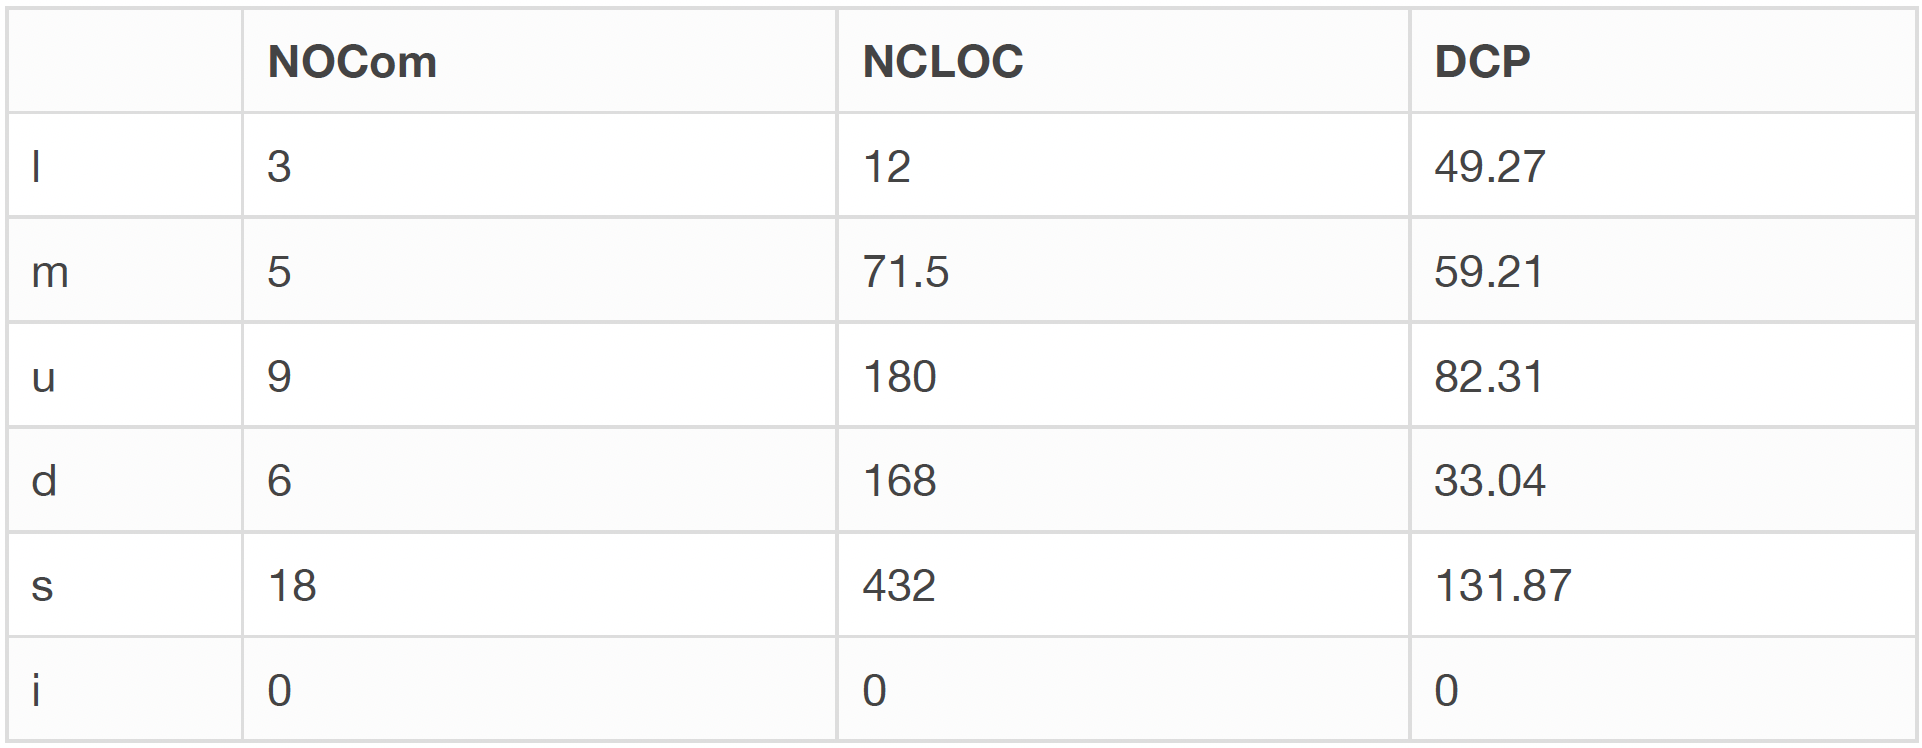
\includegraphics[scale=0.35]{T1_1.png}\\
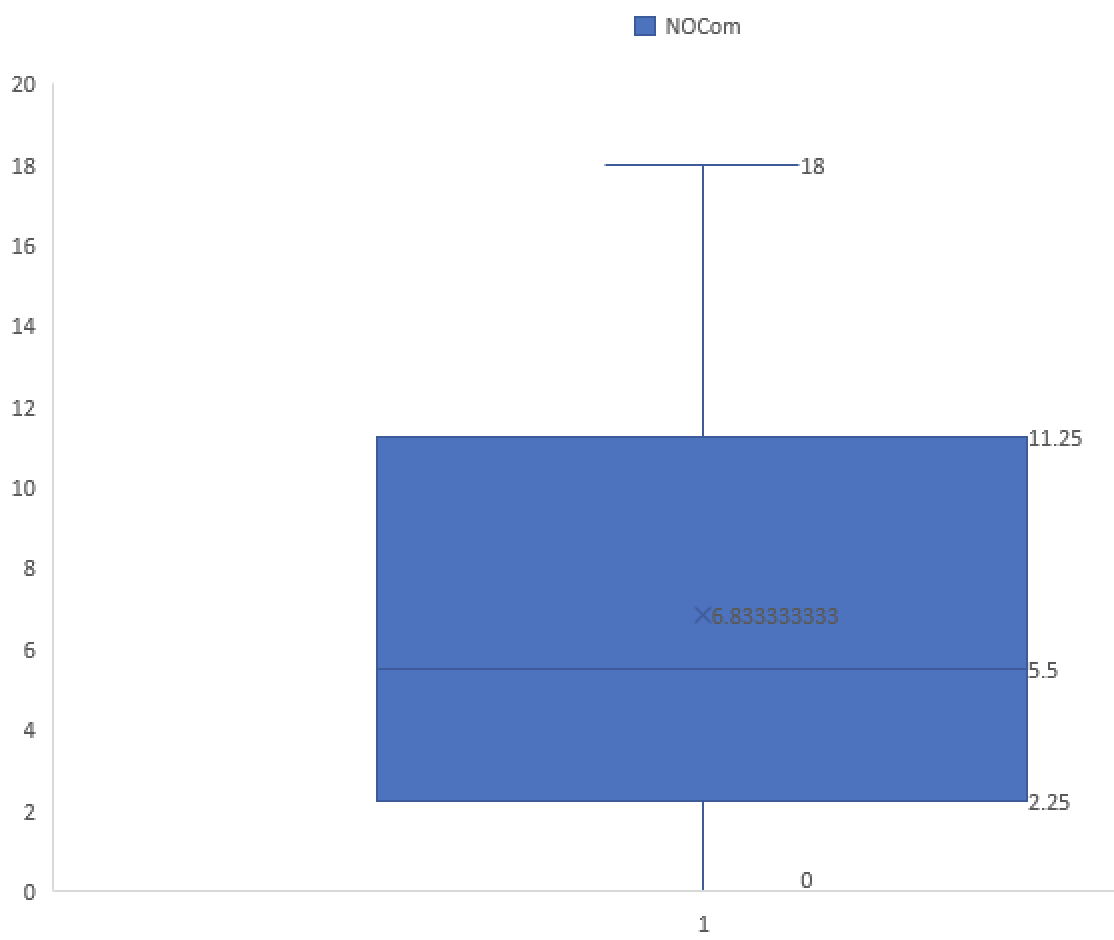
\includegraphics[scale=0.5]{NOCom.png}\\
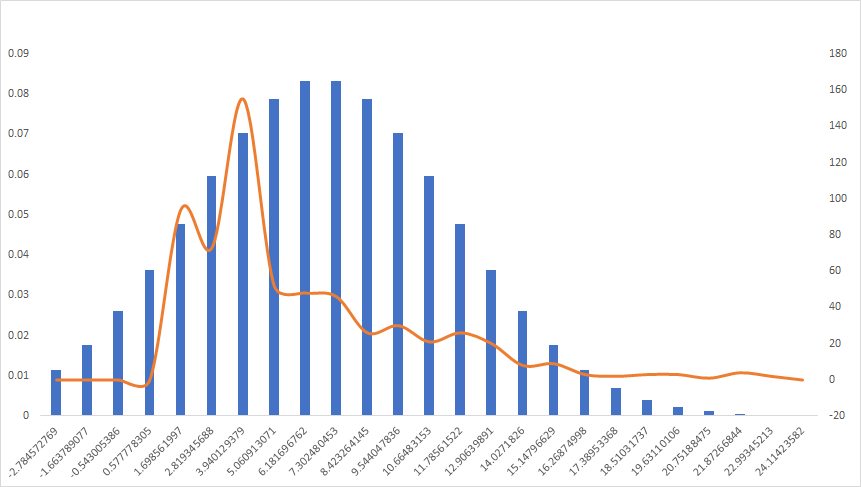
\includegraphics[scale=0.35]{T1_2.png}\\
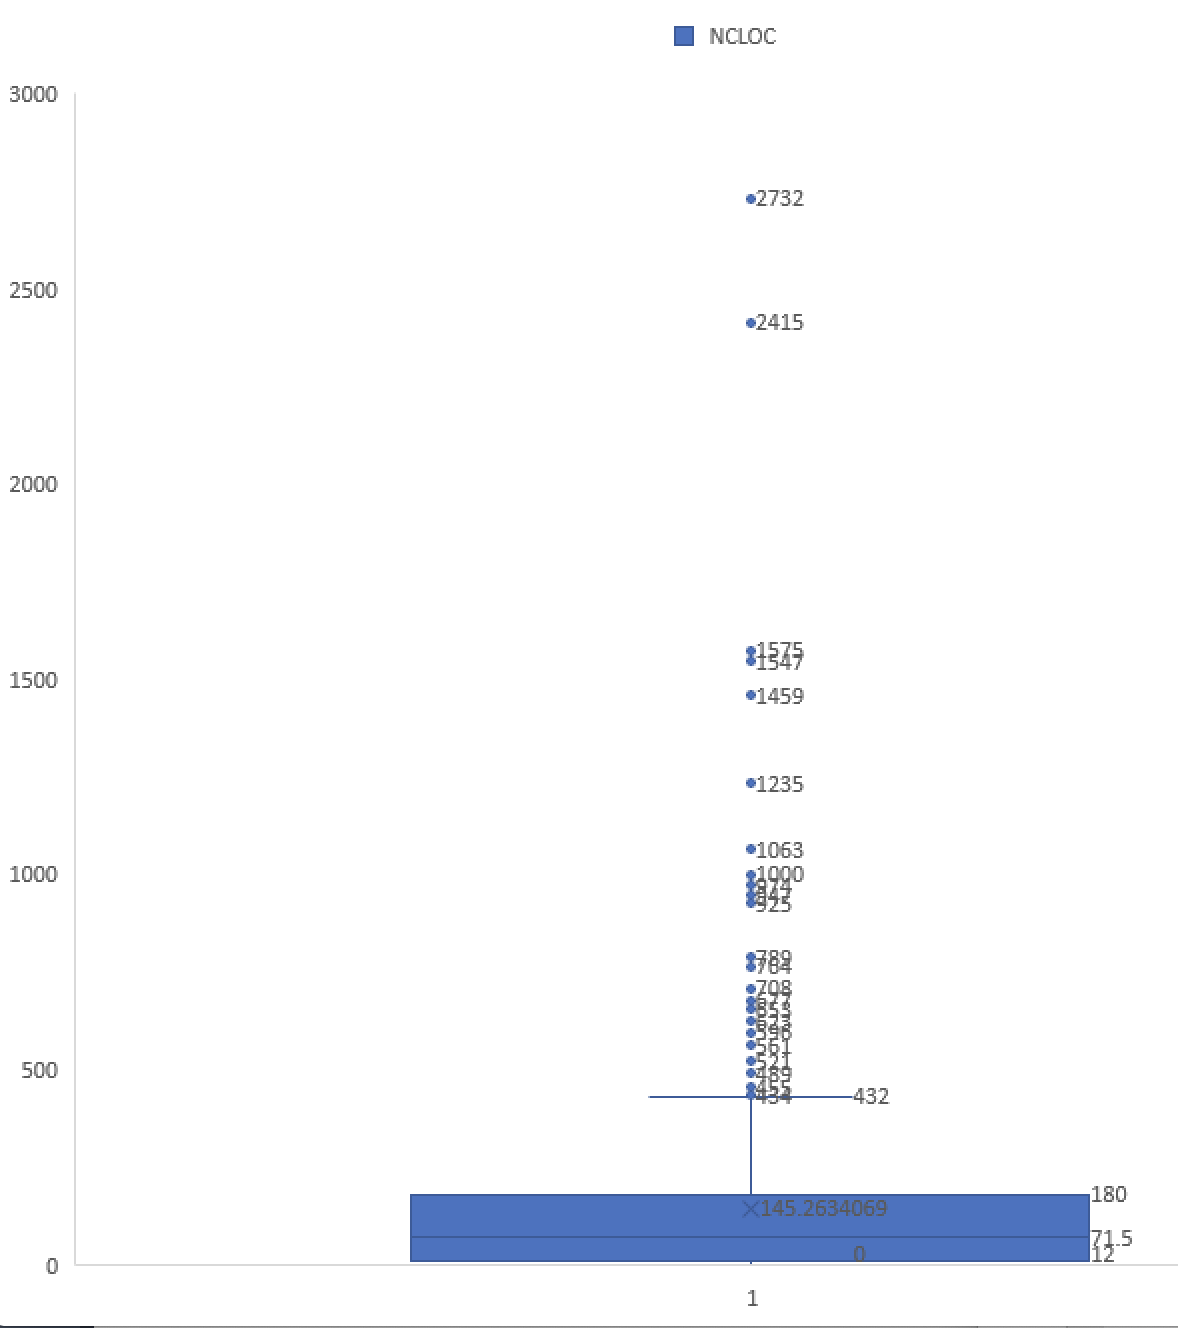
\includegraphics[scale=0.5]{NCLOC.png}
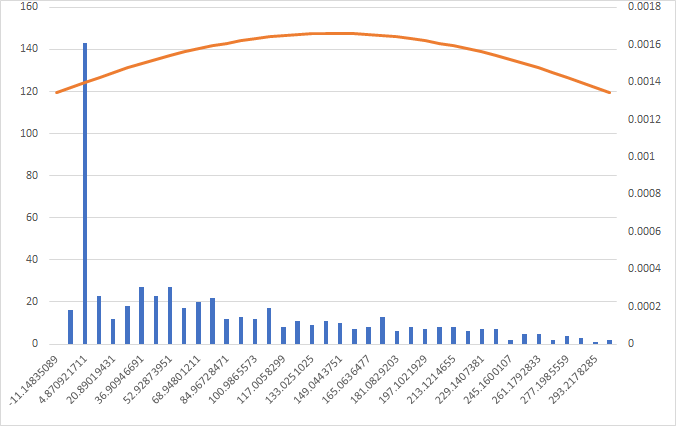
\includegraphics[scale=0.35]{T1_3.png}\\
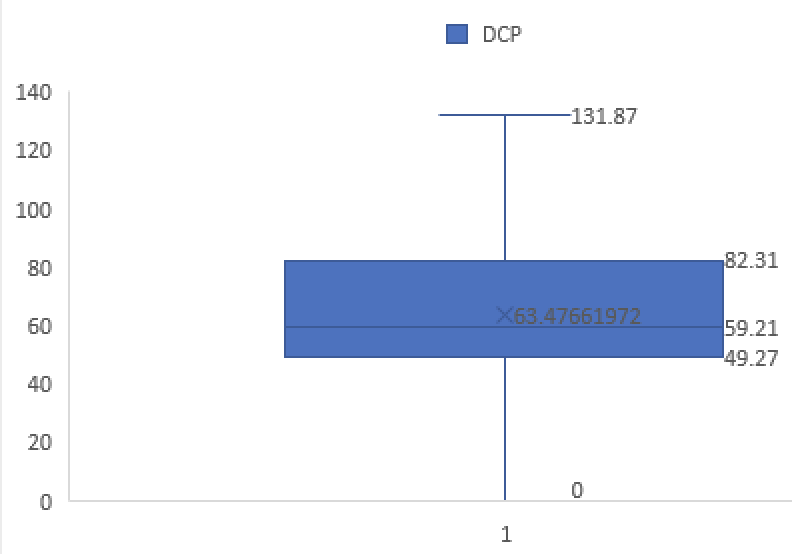
\includegraphics[scale=0.6]{DCP.png}
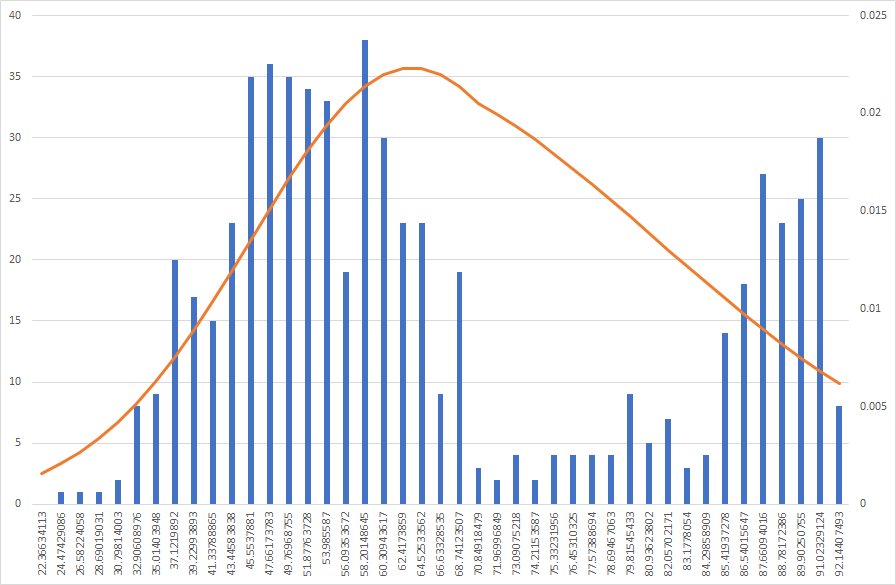
\includegraphics[scale=0.35]{T1_4.png}\\

Le tableau contient les informations nécessaires pour représenter la boîte à moustaches. À partir de la courbe de distribution, la distribution de NoCom n'est pas très proche de la distribution normale, tandis que la courbe normale de NCLOC est la meilleure, mais l'écart type est plus grand, la courbe normale de DCP est très proche de la courbe normale standard, et l'écart type est acceptable.\\


\section*{Tâche 2}\\

Coefficient de corrélation de Pearson (r):\\

r(NoCom, NCLOC) : 0.71457166 \qquad r(NoCom, DCP) : -0.487753\\

Coefficient de corrélation de rang de Spearman ($\rho$):\\

$\rho$(NoCom, NCLOC) : 0.7098611 \qquad $\rho$(NoCom, DCP) : -0.4267282\\

Courbe de régression:\\
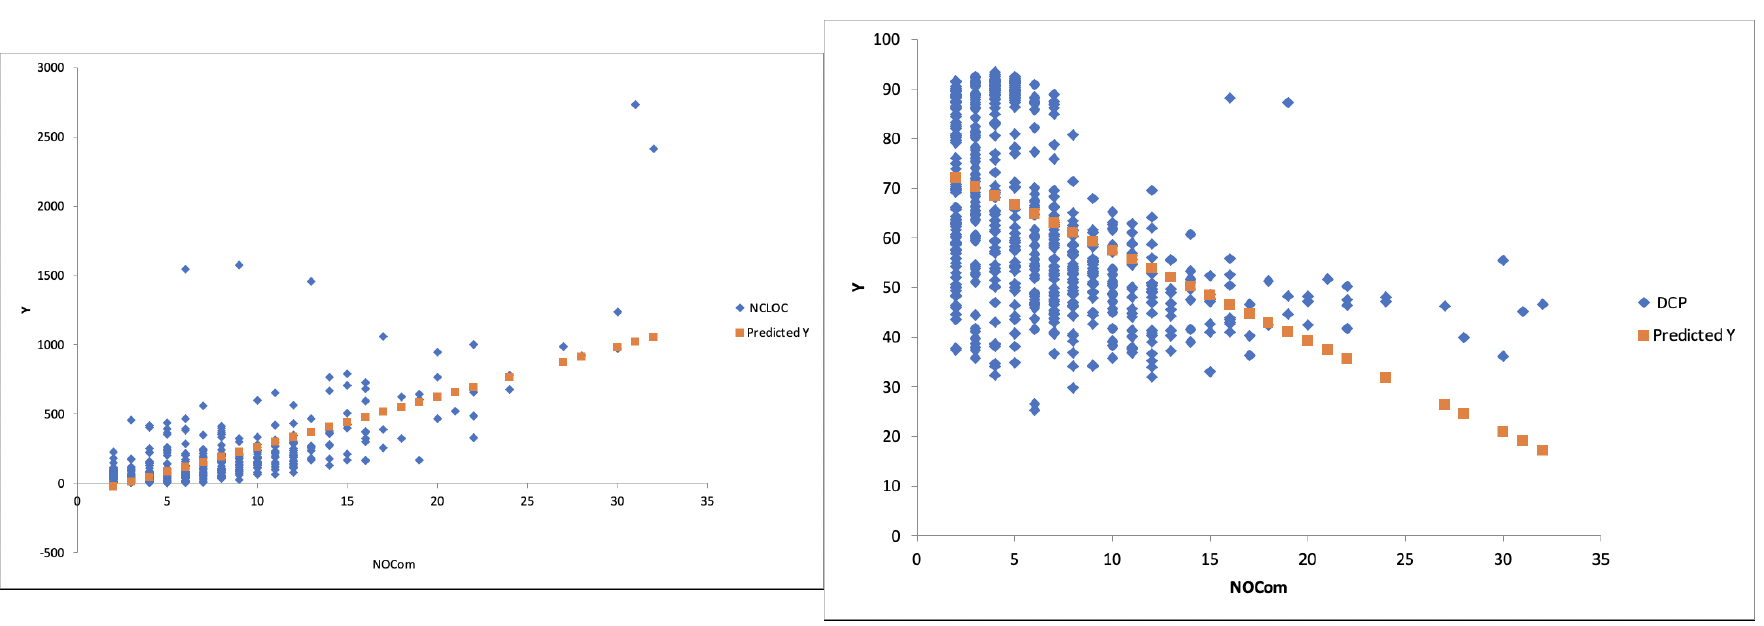
\includegraphics[scale=0.6]{T2.png}\\
Nous pouvons trouver à partir des trois indicateurs différents du coefficient de corrélation de Pearson (r), du coefficient de corrélation de rang de Spearman ($\rho$) et de la courbe de régression qu'il existe une forte corrélation positive entre NoCom et NCLOC, et une corrélation relativement forte entre NoCom et DCP Corrélation négative faible .





\section*{Tâche 3}\\
Evaluer l’hypothèse\\

\textbf{1. Choisissez le type d'étude}\\

Quasi-expérience\\

Nous savons déjà que le nombre de modifications de classe est positivement corrélé avec les lignes de code et négativement corrélé avec la densité des commentaires. Mais nous ne connaissons toujours pas la relation entre le nombre de modifications de classe et de bonnes révisions, nous voulons donc étudier la relation entre le nombre de modifications de classe et de meilleures révisions à travers des quasi-expériences.\\

\textbf{2. Définir et énoncer les hypothèses}\\

Nous faisons l'hypothèse : les classes qui ont été modifiées plus de 10 fois sont mieux commentées que celles qui ont été modifiées moins de 10 fois.\\

\textbf{3. Définir et étudier les variables}\\

NoCom\_over10 : défini comme une classe avec plus de 10 modifications. (NoCom $>$ 10)\\

NoCom\_down10 : défini comme des classes avec moins de 10 modifications. (NoCom $<$ 10)\\

Good\_comments : définis comme de bons commentaires, les bons commentaires doivent être étroitement liés au code, de sorte qu'il n'y aura pas trop de commentaires redondants, et la densité de commentaires des bons commentaires doit être faible. (1/DCP)\\

Avg\_over10 : défini comme la moyenne de good\_comments pour les classes avec plus de 10 modifications. (AVERAGE(NoCom $>$ 10, Good\_comments))\\

avg\_down10 : défini comme la moyenne de good\_comments pour les classes avec moins de 10 modifications. (AVERAGE(NoCom $<$ 10, Good\_comments))\\

\textbf{4. Interpréter et généraliser les résultats}\\

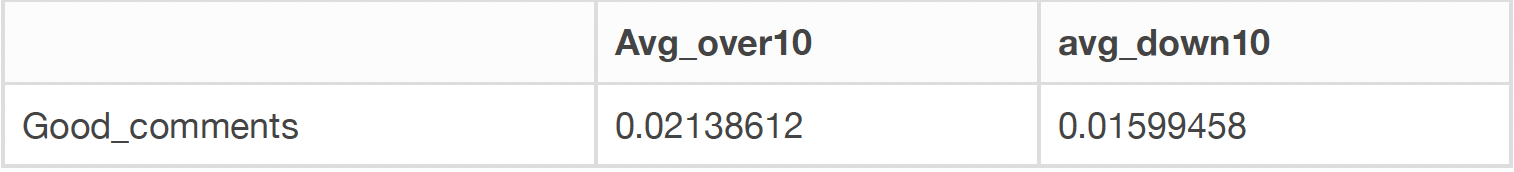
\includegraphics[scale=0.4]{T4_1.png}\\
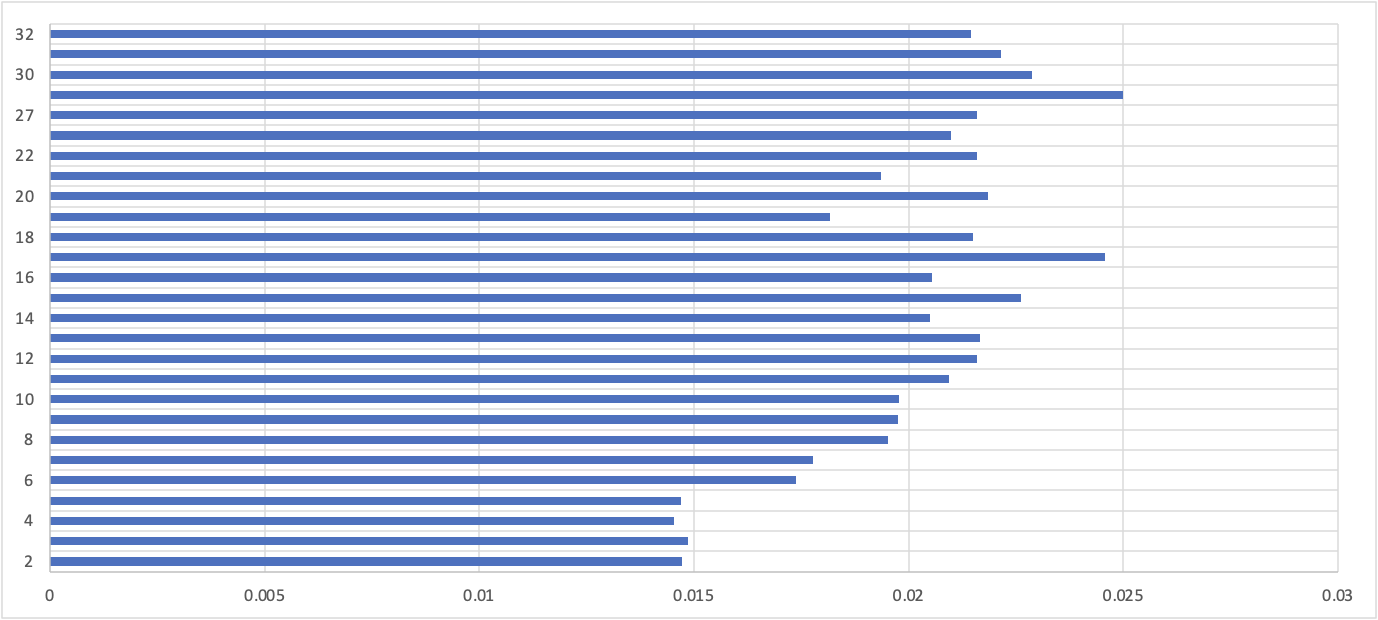
\includegraphics[scale=0.6]{T4_2.png}\\

(L'axe des ordonnées de l'histogramme est le nombre de modifications de classe NoCom, et l'axe des abscisses est le bon commentaire correspondant)\\

Dans le tableau, nous pouvons voir que le Good\_comments des classes avec plus de 10 modifications est de 0,02138612 est supérieur à 0,01599458 pour les classes avec moins de 10 modifications. Dans le même temps, nous pouvons également constater à partir de l'histogramme que les Good\_comments des classes avec plus de 10 modifications sont fondamentalement plus que celles avec moins de 10 modifications.\\

On peut donc supposer que l'hypothèse "les classes qui ont été modifiées plus de 10 fois sont mieux commentées que celles qui ont été modifiées moins de 10 fois" est correcte.\\

\textbf{5. discussion des menaces à la validité}\\

Quant à la métrique subjective des "bons commentaires", nous n'utilisons la métrique de densité de commentaires que quantitativement, en ignorant la quantité de code de la classe et la qualité réelle des commentaires.
Par conséquent, pour cette étude quasi-expérimentale, nous avons affirmé l'hypothèse proposée sur la base des indicateurs définis par nous-mêmes, et avons également eu une certaine influence sur la validité en ignorant les facteurs subjectifs et certains indicateurs potentiels internes.


\end{document}
